\documentclass{beamer}

% Theme choice
\usetheme{Madrid} % You can change to e.g., Warsaw, Berlin, CambridgeUS, etc.

% Encoding and font
\usepackage[utf8]{inputenc}
\usepackage[T1]{fontenc}

% Graphics and tables
\usepackage{graphicx}
\usepackage{booktabs}

% Code listings
\usepackage{listings}
\lstset{
basicstyle=\ttfamily\small,
keywordstyle=\color{blue},
commentstyle=\color{gray},
stringstyle=\color{red},
breaklines=true,
frame=single
}

% Math packages
\usepackage{amsmath}
\usepackage{amssymb}

% Colors
\usepackage{xcolor}

% TikZ and PGFPlots
\usepackage{tikz}
\usepackage{pgfplots}
\pgfplotsset{compat=1.18}
\usetikzlibrary{positioning}

% Hyperlinks
\usepackage{hyperref}

% Title information
\title{Week 12: Group Project Presentations}
\author{Your Name}
\institute{Your Institution}
\date{\today}

\begin{document}

\frame{\titlepage}

\begin{frame}[fragile]
    \frametitle{Introduction to Group Project Presentations}
    \begin{block}{Overview}
        Group project presentations are essential in the academic journey, showcasing collaboration and applied learning through effective communication.
    \end{block}
\end{frame}

\begin{frame}[fragile]
    \frametitle{Objectives of Group Project Presentations}
    \begin{enumerate}
        \item \textbf{Showcase Collaboration:}
            \begin{itemize}
                \item Reflects team effectiveness and diverse contributions.
                \item Demonstrates how collective efforts achieve common goals.
            \end{itemize}
        
        \item \textbf{Illustrate Applied Learning:}
            \begin{itemize}
                \item Apply theoretical knowledge to real-world problems.
                \item Solidifies understanding and retention of complex concepts.
            \end{itemize}
        
        \item \textbf{Develop Communication Skills:}
            \begin{itemize}
                \item Enhances verbal and nonverbal communication skills.
                \item Essential for clear articulation of ideas to various audiences.
            \end{itemize}

        \item \textbf{Receive Constructive Feedback:}
            \begin{itemize}
                \item Identifies strengths and areas for improvement.
                \item Fosters an environment of continuous learning and growth.
            \end{itemize}
    \end{enumerate}
\end{frame}

\begin{frame}[fragile]
    \frametitle{Importance of Student Presentations}
    \begin{itemize}
        \item \textbf{Real-World Relevance:} Prepares students for professional presentation scenarios.
        \item \textbf{Confidence Building:} Boosts self-esteem and public speaking skills.
        \item \textbf{Critical Thinking:} Requires synthesizing information and anticipating questions, enhancing analytical skills.
    \end{itemize}
\end{frame}

\begin{frame}[fragile]
    \frametitle{Key Points to Emphasize}
    \begin{itemize}
        \item Teamwork enhances analysis depth and project creativity.
        \item Engaging presentations maintain audience interest and foster dialogue.
        \item Learning through teaching solidifies personal understanding.
    \end{itemize}
\end{frame}

\begin{frame}[fragile]
    \frametitle{Conclusion}
    Group project presentations combine collaboration, application, and communication, preparing students for academic and real-world challenges.
\end{frame}

\begin{frame}[fragile]
    \frametitle{Presentation Goals - Overview}
    The primary goals of group project presentations are to effectively demonstrate teamwork, showcase the application of learned software engineering principles, and facilitate effective communication among group members and with the audience. Each goal contributes to the overall assessment of both individual and group performance.
\end{frame}

\begin{frame}[fragile]
    \frametitle{Presentation Goals - 1. Demonstrating Teamwork}
    \begin{itemize}
        \item \textbf{Concept Explanation}: Teamwork involves the collaborative effort of a group to achieve a common goal, encompassing coordination and collaboration.
        
        \item \textbf{Key Points to Emphasize}:
        \begin{itemize}
            \item \textbf{Role Distribution}: Define each member's role to highlight contributions.
            \item \textbf{Conflict Resolution}: Discuss how conflicts and decision-making challenges were resolved.
            \item \textbf{Collaboration Tools}: Mention tools used (e.g., GitHub, Trello) to enhance teamwork.
        \end{itemize}
        
        \item \textbf{Example}: A team's presentation can showcase task assignments, focusing on how members coordinated their efforts through regular meetings.
    \end{itemize}
\end{frame}

\begin{frame}[fragile]
    \frametitle{Presentation Goals - 2. Application of Learned Software Engineering Principles}
    \begin{itemize}
        \item \textbf{Concept Explanation}: Integrating theoretical knowledge and practical skills into the project.
        
        \item \textbf{Key Points to Emphasize}:
        \begin{itemize}
            \item \textbf{Design Patterns}: Discuss applied patterns (e.g., MVC, Singleton) and their justification.
            \item \textbf{Software Development Lifecycle}: Highlight adherence to phases such as design and testing.
            \item \textbf{Best Practices}: Review coding standards followed for quality assurance.
        \end{itemize}
        
        \item \textbf{Example}: A team might explain their Agile approach, focusing on adaptation to changing requirements through iterative development.
    \end{itemize}
\end{frame}

\begin{frame}[fragile]
    \frametitle{Presentation Goals - 3. Effective Communication}
    \begin{itemize}
        \item \textbf{Concept Explanation}: Clear and concise exchange of information during the presentation.
        
        \item \textbf{Key Points to Emphasize}:
        \begin{itemize}
            \item \textbf{Clear Messaging}: Ensure understandable content, minimizing jargon.
            \item \textbf{Engagement}: Involve the audience through questions and discussions.
            \item \textbf{Visual Aids}: Use visuals effectively to support verbal communication.
        \end{itemize}
        
        \item \textbf{Example}: Engage the audience by inviting questions after each segment and using flowcharts for complex processes.
    \end{itemize}
\end{frame}

\begin{frame}[fragile]
    \frametitle{Presentation Goals - Conclusion}
    By focusing on teamwork, application of engineering principles, and effective communication, students enhance their presentation skills and reflect on their collaborative experiences. Each component is crucial in preparing for real-world scenarios where these skills are vital for success.
\end{frame}

\begin{frame}[fragile]
    \frametitle{Structure of Presentations - Importance}
    \begin{itemize}
        \item A well-structured presentation ensures clarity and helps the audience follow the flow of information.
        \item It enhances teamwork by distributing roles effectively among group members.
    \end{itemize}
\end{frame}

\begin{frame}[fragile]
    \frametitle{Typical Structure of Group Presentations - Project Overview}
    \begin{block}{A. Project Overview}
        \begin{itemize}
            \item \textbf{Definition:} A brief summary of the project, including objectives and goals.
            \item \textbf{Key Points to Include:}
                \begin{itemize}
                    \item What problem does the project address?
                    \item Why is it important?
                    \item What are the main objectives?
                \end{itemize}
            \item \textbf{Example:} "Our project aims to create a mobile application that improves daily task management for students by integrating their schedules with to-do lists."
        \end{itemize}
    \end{block}
\end{frame}

\begin{frame}[fragile]
    \frametitle{Typical Structure of Group Presentations - Methodology}
    \begin{block}{B. Methodology}
        \begin{itemize}
            \item \textbf{Definition:} The approach and strategies used to tackle the project.
            \item \textbf{Key Points to Include:}
                \begin{itemize}
                    \item Which methodologies were employed? (e.g., Agile, Waterfall)
                    \item Why were they chosen?
                    \item Tools and techniques used for development.
                \end{itemize}
            \item \textbf{Example:} "We used the Agile methodology to further refine our app based on user feedback through weekly sprints."
        \end{itemize}
    \end{block}
\end{frame}

\begin{frame}[fragile]
    \frametitle{Typical Structure of Group Presentations - Implementation}
    \begin{block}{C. Implementation}
        \begin{itemize}
            \item \textbf{Definition:} The process of executing the project plan.
            \item \textbf{Key Points to Include:}
                \begin{itemize}
                    \item Workflow: Describe the steps taken during development.
                    \item Challenges faced and how they were overcome.
                    \item Division of tasks among team members.
                \end{itemize}
            \item \textbf{Example:} "The team divided tasks: Alice handled UI/UX design, while Bob focused on backend development."
            \item \textbf{Illustration:} Consider a flowchart showing the development phases (planning, coding, testing).
        \end{itemize}
    \end{block}
\end{frame}

\begin{frame}[fragile]
    \frametitle{Typical Structure of Group Presentations - Outcomes}
    \begin{block}{D. Outcomes}
        \begin{itemize}
            \item \textbf{Definition:} The results obtained from the project.
            \item \textbf{Key Points to Include:}
                \begin{itemize}
                    \item Achievements vs. initial objectives.
                    \item Any metrics or data that demonstrate success.
                    \item Feedback received from testing or user trials.
                \end{itemize}
            \item \textbf{Example:} "User testing revealed a 30\% increase in task completion rates using our app, aligning with our goal of improving productivity."
        \end{itemize}
    \end{block}
\end{frame}

\begin{frame}[fragile]
    \frametitle{Conclusion and Key Takeaways}
    \begin{itemize}
        \item Recap the importance of following a structured approach to deliver engaging and informative presentations.
        \item \textbf{Key Takeaways:} 
        \begin{itemize}
            \item Clear Flow: A structured format helps maintain a logical progression.
            \item Engagement Through Clarity: Detailed sections foster audience understanding and retention.
            \item Role Distribution: Helps utilize each team member’s strength effectively.
        \end{itemize}
    \end{itemize}
    \begin{block}{Interactive Element}
        Consider incorporating a Q\&A segment after your presentation to engage the audience further.
    \end{block}
\end{frame}

\begin{frame}[fragile]
    \frametitle{Software Engineering Principles Applied}
    \begin{block}{Key Software Engineering Principles and Methodologies}
        \begin{enumerate}
            \item Agile Methodology
            \item Waterfall Methodology
            \item Key Points to Emphasize
            \item Implementation Strategies
        \end{enumerate}
    \end{block}
\end{frame}

\begin{frame}[fragile]
    \frametitle{Agile Methodology}
    \begin{itemize}
        \item \textbf{Overview:} An iterative approach emphasizing flexibility, collaboration, and quick delivery.
        \item \textbf{Core Principles:}
        \begin{itemize}
            \item Customer satisfaction through early and continuous delivery.
            \item Welcoming changing requirements, even late in development.
            \item Emphasizing collaboration between developers and stakeholders.
            \item Frequent delivery of functional software.
        \end{itemize}
        \item \textbf{Example:} Teams may break work into "sprints" lasting 1-4 weeks for goal setting, development, and review.
    \end{itemize}
\end{frame}

\begin{frame}[fragile]
    \frametitle{Waterfall Methodology}
    \begin{itemize}
        \item \textbf{Overview:} A linear and sequential approach flowing from conception to maintenance.
        \item \textbf{Core Principles:}
        \begin{itemize}
            \item Clearly defined stages: Requirements, Design, Implementation, Verification, and Maintenance.
            \item Each stage is completed before moving to the next with less flexibility for changes once a stage is complete.
        \end{itemize}
        \item \textbf{Example:} Developing a library management system with detailed documentation required before moving to design.
    \end{itemize}
\end{frame}

\begin{frame}[fragile]
    \frametitle{Key Points and Implementation Strategies}
    \begin{itemize}
        \item \textbf{Flexibility vs. Structure:}
        \begin{itemize}
            \item Agile is flexible for dynamic projects.
            \item Waterfall is structured for projects with well-defined requirements.
        \end{itemize}
        \item \textbf{Stakeholder Involvement:}
        \begin{itemize}
            \item Agile requires ongoing collaboration.
            \item Waterfall focuses on upfront input limiting changes later.
        \end{itemize}
        \item \textbf{Choosing a Methodology:} Assess project requirements to determine the most suitable methodology.
        \item \textbf{Combining Methodologies:} Blend Agile sprints within Waterfall for flexibility along with discipline.
    \end{itemize}
\end{frame}

\begin{frame}[fragile]
    \frametitle{Conclusion and Models}
    \begin{block}{Conclusion}
        In your projects, choose methodologies that best fit your objectives—Agile for responsiveness and collaboration, or Waterfall for clear requirements.
    \end{block}
    \begin{block}{Agile Cycle}
        \begin{center}
        [Plan] $\rightarrow$ [Design] $\rightarrow$ [Develop] $\rightarrow$ [Test] $\rightarrow$ [Release] $\rightarrow$ [Review]
        \end{center}
    \end{block}
    \begin{block}{Waterfall Model}
        \begin{center}
        [Requirements] $\rightarrow$ [Design] $\rightarrow$ [Implementation] $\rightarrow$ [Verification] $\rightarrow$ [Maintenance]
        \end{center}
    \end{block}
\end{frame}

\begin{frame}[fragile]
    \frametitle{Collaborative Tools and Techniques - Introduction}
    Collaboration is essential in software development, especially during group projects. It ensures that team members can work together efficiently, share knowledge, and maintain consistency in the project.
\end{frame}

\begin{frame}[fragile]
    \frametitle{Key Collaborative Tools - Version Control Systems}
    \textbf{Example: Git}
    \begin{itemize}
        \item \textbf{Purpose}: Manages changes to source code over time.
        \item \textbf{Functionality}:
        \begin{itemize}
            \item Allow simultaneous work on the same codebase.
            \item Track history of code changes and facilitate rollbacks.
            \item Support independent feature development with branching and merging.
        \end{itemize}
    \end{itemize}
\end{frame}

\begin{frame}[fragile]
    \frametitle{Basic Git Commands}
    \begin{lstlisting}[language=bash]
git clone <repository-url>  # Copies a repository to your local machine
git add <file>               # Stages changes for the next commit
git commit -m "Message"     # Records changes with a message
git push origin <branch>     # Sends local changes to a remote repository
    \end{lstlisting}
\end{frame}

\begin{frame}[fragile]
    \frametitle{Key Collaborative Tools - Collaboration Platforms}
    \textbf{Examples: GitHub, GitLab, Bitbucket}
    \begin{itemize}
        \item \textbf{Purpose}: Online platforms for remote collaboration and version control.
        \item \textbf{Features}:
        \begin{itemize}
            \item Code reviews via pull requests.
            \item Issue tracking for project management.
            \item Documentation hosting through wikis or Markdown files.
        \end{itemize}
    \end{itemize}
\end{frame}

\begin{frame}[fragile]
    \frametitle{Key Collaborative Tools - Communication Tools}
    \textbf{Examples: Slack, Microsoft Teams, Discord}
    \begin{itemize}
        \item \textbf{Purpose}: Facilitates real-time communication among team members.
        \item \textbf{Functionality}:
        \begin{itemize}
            \item Create channels for focused discussions.
            \item Integrate with other tools like GitHub for notifications.
        \end{itemize}
    \end{itemize}
\end{frame}

\begin{frame}[fragile]
    \frametitle{Key Collaborative Tools - Project Management Tools}
    \textbf{Examples: Trello, JIRA, Asana}
    \begin{itemize}
        \item \textbf{Purpose}: Helps in planning, tracking, and managing project progress.
        \item \textbf{Functionality}:
        \begin{itemize}
            \item Visual task boards to track assignment status.
            \item User story mapping for Agile methodologies.
        \end{itemize}
    \end{itemize}
\end{frame}

\begin{frame}[fragile]
    \frametitle{Collaborative Techniques - Overview}
    \begin{block}{Regular Stand-up Meetings}
        \begin{itemize}
            \item \textbf{Purpose}: Brief daily or weekly meetings to share progress and discuss challenges.
            \item \textbf{Benefits}:
            \begin{itemize}
                \item Keeps the team aligned and informed.
                \item Identifies potential roadblocks early.
            \end{itemize}
        \end{itemize}
    \end{block}
\end{frame}

\begin{frame}[fragile]
    \frametitle{Collaborative Techniques - Pair Programming}
    \begin{block}{Purpose and Benefits}
        \begin{itemize}
            \item \textbf{Purpose}: Two programmers work on the same code.
            \item \textbf{Benefits}:
            \begin{itemize}
                \item Enhances code quality and encourages knowledge sharing.
                \item Balances expertise levels within the team.
            \end{itemize}
        \end{itemize}
    \end{block}
\end{frame}

\begin{frame}[fragile]
    \frametitle{Collaborative Techniques - Code Reviews}
    \begin{block}{Purpose and Benefits}
        \begin{itemize}
            \item \textbf{Purpose}: Team members review each other's code before merging changes.
            \item \textbf{Benefits}:
            \begin{itemize}
                \item Reduces bugs and improves code quality.
                \item Promotes best practices and learning opportunities.
            \end{itemize}
        \end{itemize}
    \end{block}
\end{frame}

\begin{frame}[fragile]
    \frametitle{Key Points to Emphasize and Conclusion}
    \begin{itemize}
        \item Effective collaboration improves productivity and fosters innovation.
        \item Choose tools that fit your team's workflow and project requirements.
        \item Encourage an open communication culture for smoother collaboration.
    \end{itemize}
    
    Utilizing the right tools and techniques enhances collaboration, improves quality, and leads to successful outcomes.
\end{frame}

\begin{frame}
    \frametitle{Quality Assurance Practices}
    Quality Assurance (QA) is a systematic process to ensure that a product meets specified requirements, is dependable, satisfactory, and safe. In software development, QA is critical for functionality and user experience.
\end{frame}

\begin{frame}
    \frametitle{Key QA Methods Employed}
    \begin{enumerate}
        \item \textbf{Unit Testing}
        \begin{itemize}
            \item \textbf{Definition}: Testing individual components to ensure they work correctly.
            \item \textbf{Purpose}: Validate correctness and catch bugs early in development.
            \item \textbf{Example}:
            \begin{lstlisting}[language=Python]
def add(a, b):
    return a + b

# Unit Test for add function
def test_add():
    assert add(2, 3) == 5
    assert add(-1, 1) == 0
            \end{lstlisting}
            \item \textbf{Best Practices}:
            \begin{itemize}
                \item Write tests alongside code (Test-Driven Development).
                \item Aim for high code coverage.
            \end{itemize}
        \end{itemize}

        \item \textbf{Documentation Principles}
        \begin{itemize}
            \item \textbf{Importance}: Critical for code maintenance and team onboarding.
            \item \textbf{Types of Documentation}:
            \begin{itemize}
                \item Code Documentation
                \item Technical Documentation
                \item User Documentation
            \end{itemize}
            \item \textbf{Documentation Tools}: Markdown, JSDoc.
        \end{itemize}
    \end{enumerate}
\end{frame}

\begin{frame}
    \frametitle{Illustrating QA Practices}
    \begin{block}{The QA Process Cycle}
    \begin{center}
    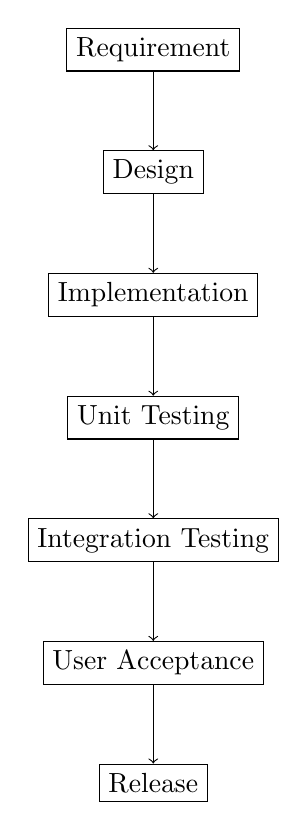
\begin{tikzpicture}
        \node (req) [draw] {Requirement};
        \node (design) [draw, below=of req] {Design};
        \node (implementation) [draw, below=of design] {Implementation};
        \node (unitTest) [draw, below=of implementation] {Unit Testing};
        \node (integrationTest) [draw, below=of unitTest] {Integration Testing};
        \node (userAccept) [draw, below=of integrationTest] {User Acceptance};
        \node (release) [draw, below=of userAccept] {Release};

        \foreach \i/\j in {req/design, design/implementation, implementation/unitTest, unitTest/integrationTest, integrationTest/userAccept, userAccept/release} {
            \draw[->] (\i) -- (\j);
        }
    \end{tikzpicture}
    \end{center}
    \end{block}
\end{frame}

\begin{frame}[fragile]
    \frametitle{Addressing Ethical Considerations - Introduction}
    Ethics in software engineering encompasses the moral principles guiding the design, development, and utilization of software. 
    As future professionals, understanding these ethical considerations is essential for maintaining trust and integrity in technology-centric projects.
\end{frame}

\begin{frame}[fragile]
    \frametitle{Key Ethical Issues to Address}
    \begin{enumerate}
        \item \textbf{Privacy}:
        \begin{itemize}
            \item Users' data should be handled with utmost confidentiality.
            \item \textit{Example:} If your project involves handling user login information, encrypt all data to safeguard against unauthorized access.
        \end{itemize}

        \item \textbf{Intellectual Property}:
        \begin{itemize}
            \item Acknowledge the originality of code and ideas.
            \item \textit{Example:} If reusing libraries or frameworks, ensure they are properly attributed and comply with licensing agreements.
        \end{itemize}
        
        \item \textbf{Security}:
        \begin{itemize}
            \item Protect software from vulnerabilities and ensure safe user interactions.
            \item \textit{Example:} Regularly update your software to patch security flaws and avoid exposing user data to threats.
        \end{itemize}
        
        \item \textbf{Accessibility}:
        \begin{itemize}
            \item Ensure software is usable for people of all abilities and disabilities.
            \item \textit{Example:} Incorporate features that allow screen readers to navigate your software efficiently.
        \end{itemize}
        
        \item \textbf{Responsibility}:
        \begin{itemize}
            \item Engineers must accept responsibility for the implications of their designs.
            \item \textit{Example:} Conduct ethical impact assessments during the development phase to anticipate potential misuse.
        \end{itemize}
    \end{enumerate}
\end{frame}

\begin{frame}[fragile]
    \frametitle{Approaches Taken in Group Projects}
    \begin{itemize}
        \item \textbf{Code Ethics Review}: 
        Teams established peer review sessions specifically to evaluate ethical adherence in coding practices, ensuring compliance with ethical guidelines.

        \item \textbf{Incorporation of Ethical Frameworks}:
        Implemented frameworks like the ACM Code of Ethics to guide decision-making processes throughout project development.

        \item \textbf{Stakeholder Engagement}:
        Inviting feedback from potential users and affected groups during the planning stage, addressing their concerns to shape a more responsible outcome.

        \item \textbf{Documentation of Ethical Considerations}:
        Including a dedicated section in project documentation outlining ethical decisions made and the rationale behind them.
    \end{itemize}
\end{frame}

\begin{frame}[fragile]
    \frametitle{Technical Documentation}
    \begin{block}{Understanding Technical Documentation}
        Technical documentation refers to comprehensive materials that explain the functionality, architecture, and processes related to a software project. It serves as a guide for developers, stakeholders, and end-users, ensuring clarity and consistency throughout project development and maintenance.
    \end{block}
\end{frame}

\begin{frame}[fragile]
    \frametitle{Importance of Clear Technical Documentation - Part 1}
    \begin{itemize}
        \item \textbf{Facilitates Communication:}
        \begin{itemize}
            \item Role in Presentations: Provides a common language for team members and stakeholders, aiding collaboration and reducing misunderstandings.
            \item Example: Use of consistent terminology when describing software features prevents confusion about their functions.
        \end{itemize}
        
        \item \textbf{Supports Project Clarity:}
        \begin{itemize}
            \item Clear documentation outlines project scope, specifications, and requirements, aiding understanding of project goals.
            \item Illustration: A table listing features, requirements, and their respective statuses helps team members quickly assess progress.
        \end{itemize}
    \end{itemize}
\end{frame}

\begin{frame}[fragile]
    \frametitle{Importance of Clear Technical Documentation - Part 2}
    \begin{itemize}
        \item \textbf{Aids in Onboarding and Training:}
        \begin{itemize}
            \item New team members can refer to documentation to get up to speed on processes and existing code.
            \item Example: A dedicated onboarding guide provides an overview of coding standards, tools used, and team practices.
        \end{itemize}
        
        \item \textbf{Enhances Maintainability:}
        \begin{itemize}
            \item Clear documentation allows for easier updates and modifications. Well-documented code can quickly adapt to changes.
            \item Key Point: Documentation must be updated to reflect changes as projects evolve.
        \end{itemize}
        
        \item \textbf{Enables Effective Presentations:}
        \begin{itemize}
            \item Well-structured documentation can serve as visual aids during presentations, clarifying complex concepts.
            \item Example: Incorporating snippets of technical documents (e.g., system architecture diagrams) during the presentation can clarify complex concepts.
        \end{itemize}
    \end{itemize}
\end{frame}

\begin{frame}[fragile]
    \frametitle{Key Elements of Effective Technical Documentation}
    \begin{itemize}
        \item \textbf{Clarity:} Use simple language and avoid jargon.
        \item \textbf{Detail:} Provide enough information to guide users without overwhelming.
        \item \textbf{Structure:} Organize information logically using headings, bullet points, and tables.
        \item \textbf{Accessibility:} Ensure documentation is easy to access and navigate.
    \end{itemize}
\end{frame}

\begin{frame}[fragile]
    \frametitle{Conclusion}
    \begin{block}{Summary}
        In summary, technical documentation is essential for successful group project presentations. It:
        \begin{itemize}
            \item Ensures effective communication.
            \item Supports project clarity.
            \item Offers onboarding assistance.
            \item Enhances maintainability.
            \item Serves as a valuable resource during presentations.
        \end{itemize}
    \end{block}
    Make sure each team member understands their role in creating and maintaining technical documentation to enhance overall project success!
\end{frame}

\begin{frame}[fragile]
    \frametitle{Feedback and Peer Review Process - Overview}
    \begin{block}{Understanding Peer Feedback Mechanisms}
        Peer feedback is an evaluative process in which students provide constructive criticism on each other's work. It encourages collaborative learning and fosters critical thinking skills by allowing students to access diverse perspectives.
    \end{block}
\end{frame}

\begin{frame}[fragile]
    \frametitle{Feedback Mechanisms During Presentations}
    \begin{enumerate}
        \item \textbf{Structured Rubrics:}
        \begin{itemize}
            \item Provides clear criteria for assessing presentations (e.g., content, delivery).
            \item Categories: Clarity of Information, Use of Visual Aids, Engagement with Audience (scored 1-5).
        \end{itemize}
        
        \item \textbf{Feedback Forms:}
        \begin{itemize}
            \item Handouts or online formats for writing comments based on the rubric.
            \item Prompts: "What did you like most?" and "What could be improved?"
        \end{itemize}
        
        \item \textbf{Verbal Feedback Sessions:}
        \begin{itemize}
            \item Open discussions facilitating instant feedback after presentations.
            \item Example: Q\&A session facilitated by the instructor.
        \end{itemize}
        
        \item \textbf{Anonymous Peer Reviews:}
        \begin{itemize}
            \item Enables honest feedback without identification.
            \item Utilizes online survey tools for anonymous collection.
        \end{itemize}
    \end{enumerate}
\end{frame}

\begin{frame}[fragile]
    \frametitle{Value of Feedback in Learning Outcomes}
    \begin{enumerate}
        \item \textbf{Encourages Active Learning:} Involves students in evaluation, fostering engagement.
        \item \textbf{Develops Critical Thinking:} Analyzing presentations enhances critical assessment skills.
        \item \textbf{Fosters a Growth Mindset:} Mistakes seen as learning opportunities encourage improvement.
        \item \textbf{Improves Presentation Skills:} Adapting styles based on feedback leads to better public speaking.
        \item \textbf{Nurtures Collaborative Skills:} Encourages teamwork and respect for diverse viewpoints.
    \end{enumerate}
\end{frame}

\begin{frame}[fragile]
    \frametitle{Key Takeaways and Conclusion}
    \begin{itemize}
        \item Feedback isn’t just criticism; it’s a tool for growth.
        \item Engagement in feedback enhances retention and understanding.
        \item Creating a safe space for feedback maximizes learning potential.
    \end{itemize}

    \begin{block}{Conclusion}
        The feedback and peer review process is vital for creating an enriching educational experience.
    \end{block}
\end{frame}

\begin{frame}[fragile]
    \frametitle{Conclusion and Reflection - Part 1}
    \begin{block}{Introduction}
        As we wrap up our group project presentations, it's essential to reflect on the experiences and lessons learned throughout this process. This stage not only reinforces the knowledge gained but also emphasizes the importance of collaboration and application of software engineering concepts.
    \end{block}
\end{frame}

\begin{frame}[fragile]
    \frametitle{Conclusion and Reflection - Part 2}
    \begin{block}{Key Takeaways from the Presentations}
        \begin{enumerate}
            \item \textbf{Collaboration and Team Dynamics:}
            \begin{itemize}
                \item Group projects highlight the importance of teamwork. Effective communication, assigned roles, and shared responsibilities ensure successful project execution.
                \item \textbf{Example:} Teams that held regular meetings and utilized management tools (like Trello or Asana) performed better in aligning goals and meeting deadlines.
            \end{itemize}

            \item \textbf{Application of Software Engineering Practices:}
            \begin{itemize}
                \item Presentations demonstrated practical application of software engineering concepts like Agile methodology, version control (using Git), and testing strategies.
                \item \textbf{Example:} Teams using Agile demonstrated flexibility in adapting to feedback and iterating on designs, resulting in high-quality outcomes.
            \end{itemize}

            \item \textbf{Problem-Solving and Critical Thinking:}
            \begin{itemize}
                \item Many projects faced unforeseen challenges, requiring groups to employ critical thinking and innovative problem-solving methods.
                \item \textbf{Illustration:} A group facing a technical bug may have engaged in quick brainstorming, leading to an updated algorithm that improved application efficiency.
            \end{itemize}
        \end{enumerate}
    \end{block}
\end{frame}

\begin{frame}[fragile]
    \frametitle{Conclusion and Reflection - Part 3}
    \begin{block}{Encouraging Reflective Thinking}
        \begin{itemize}
            \item \textbf{Self-Assessment Questions:}
            \begin{itemize}
                \item What were the strengths and weaknesses of your group dynamics? 
                \item How did the group handle conflicting ideas or solutions?
                \item What software engineering principles were most applicable to your project’s success?
            \end{itemize}
            \item \textbf{Personal Growth:}
                \begin{itemize}
                    \item Reflect on your contributions and areas for development. Consider how these lessons will influence your future projects.
                \end{itemize}
            \item \textbf{Real-World Connection:}
                \begin{itemize}
                    \item Discuss how the skills and experiences gained during this project relate to real-world software development environments.
                \end{itemize}
        \end{itemize}
    \end{block}
\end{frame}

\begin{frame}[fragile]
    \frametitle{Conclusion and Reflection - Final Thoughts}
    \begin{block}{Conclusion}
        The culmination of your projects is not the end of your learning journey but a stepping stone towards becoming competent software developers. By reflecting on your experiences and the software engineering principles applied, you pave the way for ongoing growth and success in your future endeavors. 
    \end{block}
    \begin{block}{Thank You!}
        Thank you for your dedication!
    \end{block}
\end{frame}


\end{document}